\documentclass{article}
\usepackage{iclr2026_conference,times}
\input{math_commands.tex}
\usepackage{hyperref}
\usepackage{url}
\usepackage{booktabs}
\usepackage{graphicx}

\title{Visuotactile World-Model Disagreement:\\A MuJoCo Negative Result}
\author{Anonymous Authors}

\begin{document}
\maketitle

\begin{abstract}
This paper records a negative result for a tempting multimodal robotics mechanism: preserving vision-touch disagreement as explicit world-model branches during contact-rich planning.
The hypothesis is that branch preservation should outperform branch-collapsing fusion and generic uncertainty methods when hidden physical modes make vision and touch disagree.
We rebuilt the idea as a MuJoCo planar manipulation benchmark with real contact rollouts, hidden friction, visual bias, tactile noise, sticky contact, combined shift, strong non-oracle baselines, ablations, stress sweeps, and seed-level uncertainty.
The mechanism fails the submission gate.
On the combined shift, the proposed visuotactile disagreement branch planner reaches 0.450 success, while mean fusion reaches 0.667, ensemble uncertainty reaches 0.733, and an oracle reaches 0.800.
Ablations that remove branch preservation, the disagreement trigger, the risk penalty, or tactile residual updates match or beat the full method.
We therefore mark this project \textbf{KILL/ARCHIVE} for ICLR main rather than polishing an unsupported claim.
\end{abstract}

\section{Question}
Vision and touch often disagree in contact-rich robotics: vision may see an object at the wrong pose under occlusion, while touch may observe a contact force consistent with a different physical mode.
The original research bet was that a world model should not immediately average those signals.
Instead, it should keep action-critical alternatives explicit until probing or motion collapses them.
This idea sits near crowded multimodal robot-learning work on vision-touch representation learning, visual-tactile manipulation, and large robot policy models~\citep{prior4,prior7,prior8}.
The novelty boundary is therefore narrow: the mechanism must change closed-loop decisions, not merely rename uncertainty.

\section{Benchmark}
We implemented a lightweight MuJoCo pusher benchmark.
Each episode contains a sliding object, a controlled pusher, a tactile probe, a target, and a final push.
The executed actions are real MuJoCo contact rollouts.
The hidden physical split changes object friction, contact drag, vision bias, tactile noise, actuator effectiveness, or combinations of these factors.
The seven main splits are nominal, high friction, low friction, vision bias, tactile noise, sticky contact, and combined shift.

We compare nine planners.
\texttt{random\_push} is a sanity check.
\texttt{vision\_only\_mpc} and \texttt{tactile\_only\_mpc} use one modality.
\texttt{mean\_fusion\_mpc} collapses vision and touch into one state.
\texttt{ensemble\_uncertainty\_mpc} evaluates sampled physical hypotheses with a variance penalty.
\texttt{conformal\_risk\_filter} shortens or rejects high-risk actions under residual thresholds.
\texttt{diagnostic\_probe\_then\_mpc} always performs an extra probe.
\texttt{vt\_disagreement\_branch\_mpc} is the proposed method: it preserves visual, tactile, and high-force branches when the modalities disagree.
\texttt{oracle\_mode\_mpc} is a non-submission upper bound with access to the hidden mode.

\section{Results}
The main experiment uses 5 seeds, 12 episodes per seed, 7 splits, and 9 methods, producing 3,780 MuJoCo episodes.
The ablation suite adds 420 episodes and the stress sweep adds 1,200 episodes.
Success means the object ends within 7.5 cm of the target.
We also report final error, an energy/contact-effort proxy, and contact-violation rates.

\begin{table}[t]
\centering
\caption{Combined-shift results. The proposed branch planner is below strong non-oracle baselines.}
\label{tab:combined}
\begin{tabular}{lcccc}
\toprule
Method & Success & 95\% CI & Error & Energy \\
\midrule
\texttt{random\_push} & 0.083 & 0.071 & 0.151 & 0.415 \\
\texttt{vision\_only\_mpc} & 0.550 & 0.127 & 0.073 & 0.527 \\
\texttt{tactile\_only\_mpc} & 0.633 & 0.123 & 0.074 & 0.501 \\
\texttt{mean\_fusion\_mpc} & 0.667 & 0.120 & 0.064 & 0.502 \\
\texttt{ensemble\_uncertainty\_mpc} & 0.733 & 0.113 & 0.064 & 0.513 \\
\texttt{conformal\_risk\_filter} & 0.583 & 0.126 & 0.077 & 0.483 \\
\texttt{diagnostic\_probe\_then\_mpc} & 0.633 & 0.123 & 0.070 & 0.601 \\
\texttt{vt\_disagreement\_branch\_mpc} & 0.450 & 0.127 & 0.094 & 0.564 \\
\texttt{oracle\_mode\_mpc} & 0.800 & 0.102 & 0.052 & 0.554 \\
\bottomrule
\end{tabular}
\end{table}

\begin{figure}[t]
\centering
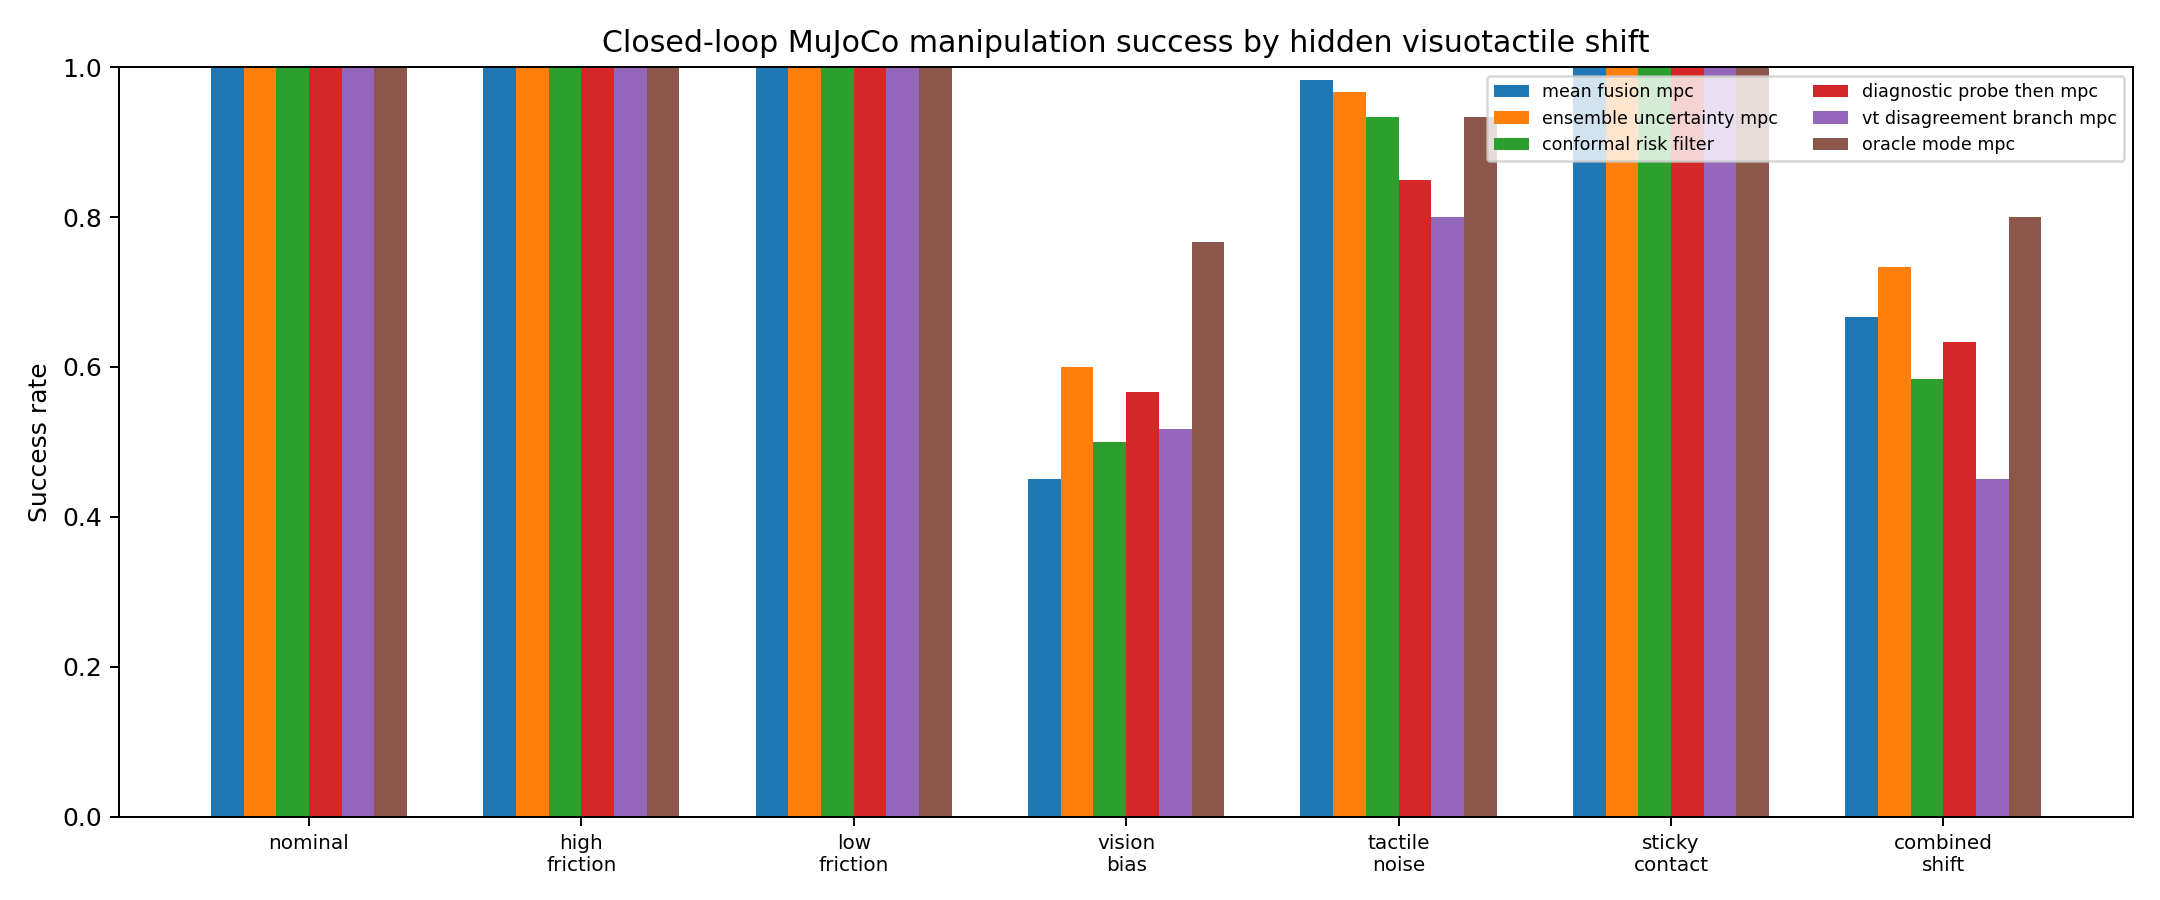
\includegraphics[width=\linewidth]{../figures/vt_disagreement_success_by_split.png}
\caption{Success across hidden visuotactile shifts. The proposed branch method does not produce a broad advantage.}
\label{fig:success}
\end{figure}

Table~\ref{tab:combined} is the central result.
On the combined shift, \texttt{vt\_disagreement\_branch\_mpc} is worse than mean fusion by 0.217 success and worse than ensemble uncertainty by 0.283 success.
Pairwise seed-level comparisons give approximate normal-test $p$ values of 0.0080 versus mean fusion and 0.0083 versus ensemble uncertainty, both in the wrong direction for the proposed method.
The oracle remains higher, showing that hidden mode information is useful, but the proposed disagreement representation is not the right way to recover it.

\section{Ablations}
\begin{table}[t]
\centering
\caption{Combined-shift ablations. Removing the claimed mechanism does not hurt.}
\label{tab:ablations}
\begin{tabular}{lccc}
\toprule
Ablation & Success & 95\% CI & Energy \\
\midrule
\texttt{full\_vt\_disagreement\_branch\_mpc} & 0.500 & 0.128 & 0.532 \\
\texttt{no\_branch\_preservation} & 0.517 & 0.128 & 0.547 \\
\texttt{no\_diagnostic\_value} & 0.550 & 0.127 & 0.481 \\
\texttt{no\_disagreement\_trigger} & 0.583 & 0.126 & 0.496 \\
\texttt{no\_risk\_penalty} & 0.600 & 0.125 & 0.523 \\
\texttt{no\_tactile\_residual\_update} & 0.767 & 0.108 & 0.519 \\
\texttt{small\_branch\_set} & 0.500 & 0.128 & 0.527 \\
\bottomrule
\end{tabular}
\end{table}

\begin{figure}[t]
\centering
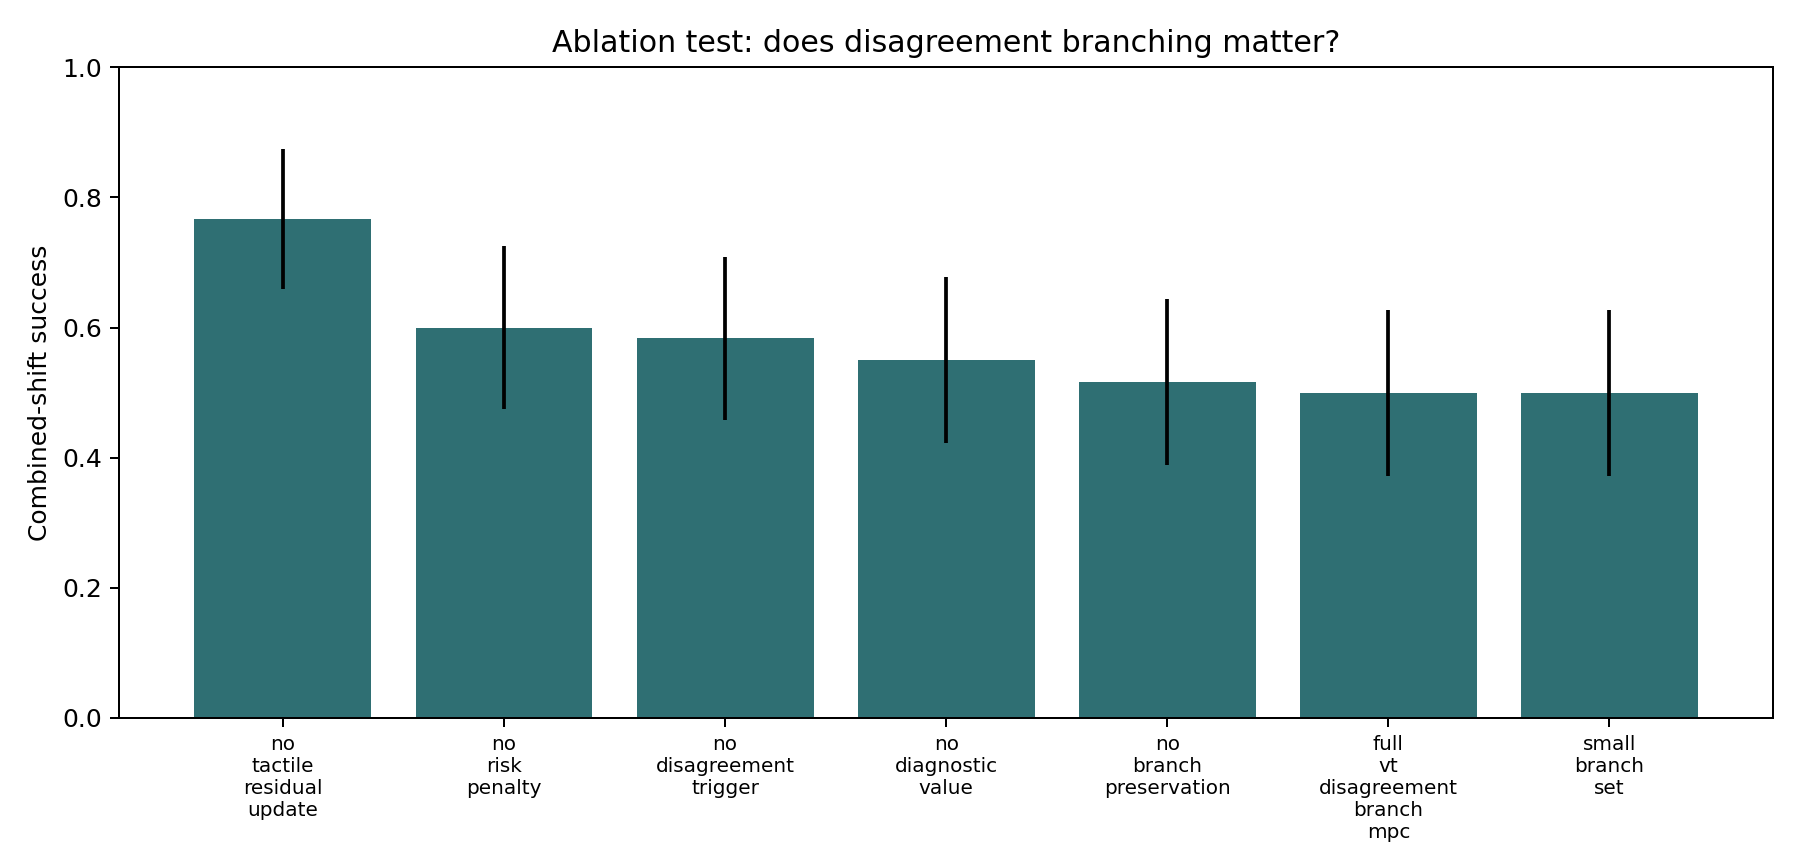
\includegraphics[width=0.88\linewidth]{../figures/vt_disagreement_ablation_success.png}
\caption{Ablations on the combined shift. The full branch mechanism is not necessary for success.}
\label{fig:ablation}
\end{figure}

The ablations are more damaging than the baseline table.
If the paper's mechanism were correct, removing branch preservation or the disagreement trigger should reduce performance.
Instead, \texttt{no\_branch\_preservation}, \texttt{no\_diagnostic\_value}, \texttt{no\_disagreement\_trigger}, \texttt{no\_risk\_penalty}, and \texttt{no\_tactile\_residual\_update} all match or beat the full method.
The tactile residual ablation is especially revealing: in this benchmark, the branch update over-trusts noisy tactile alternatives and harms planning more than it helps.

\section{Stress Tests and Negative Cases}
\begin{figure}[t]
\centering
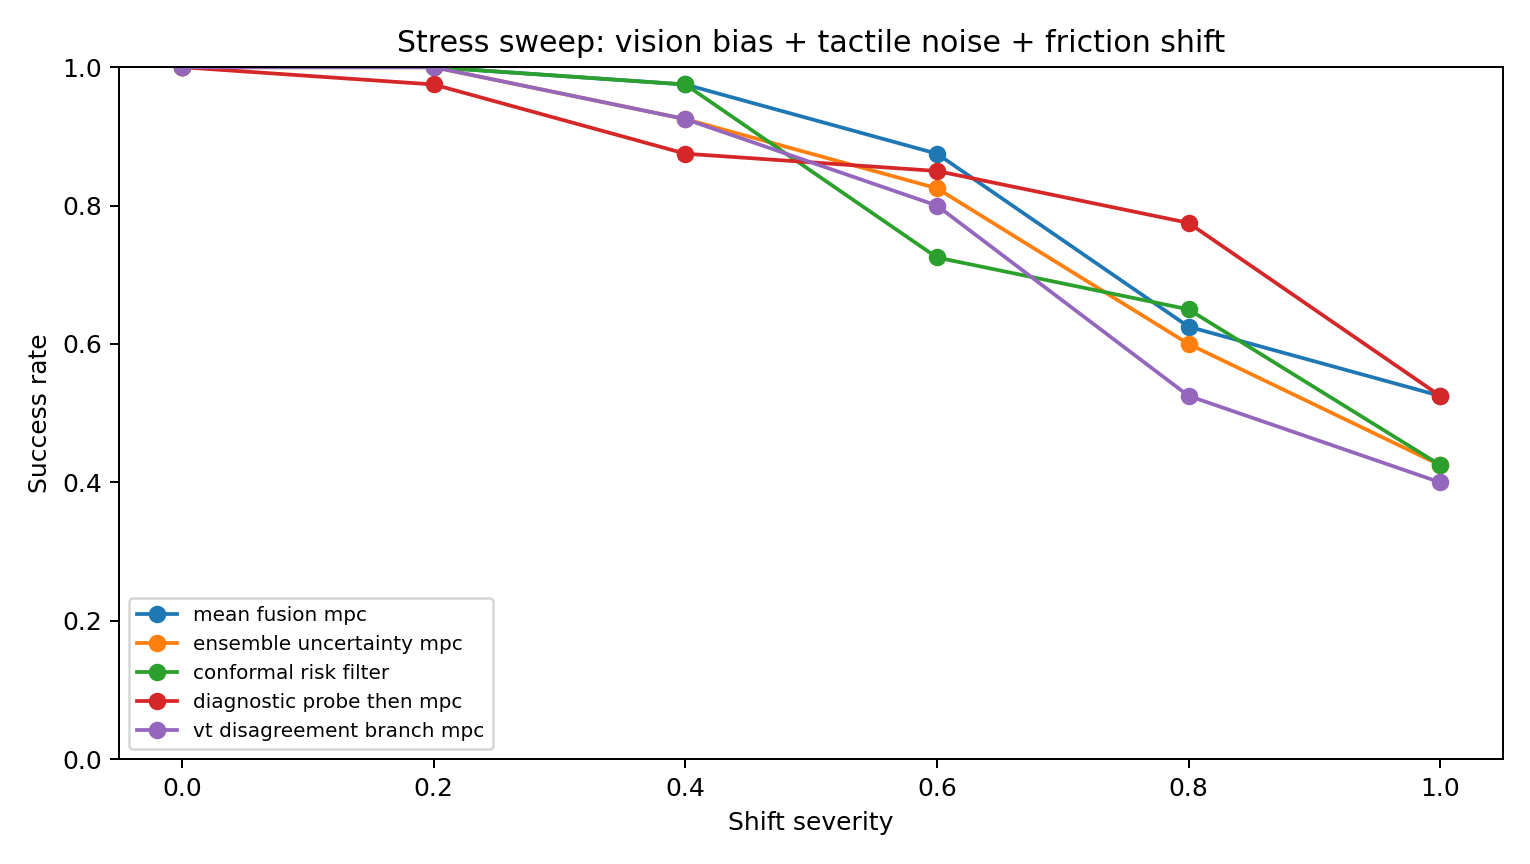
\includegraphics[width=0.82\linewidth]{../figures/vt_disagreement_stress_sweep.png}
\caption{Stress sweep over visual bias, tactile noise, and friction shift. The branch planner does not dominate robust alternatives.}
\label{fig:stress}
\end{figure}

The stress sweep jointly increases visual bias, tactile noise, and friction shift.
At maximum stress, mean fusion and diagnostic probing both reach 0.525 success, while the proposed method reaches 0.400.
We also record three negative cases: simultaneous adversarial vision and tactile corruption, unmodeled actuator weakness, and semantic target ambiguity.
These are not minor engineering issues.
They expose missing state variables that branch-preserving visuotactile disagreement does not represent.

\section{Limitations}
This is not a real-robot study.
It is a high-fidelity simulator rebuild with compact analytic planners rather than trained deep world-action models.
The related-work audit is still based on local hostile pool slices rather than a full manual review.
Those limitations would normally justify a strong-revise decision if the mechanism had produced a clear empirical signal.
It did not.
The negative conclusion therefore does not claim that all visuotactile branching is useless; it only rejects this implementation and paper thesis as an ICLR-main submission.

\section{Decision}
The submission gate was explicit: the proposed method needed to beat mean fusion, uncertainty/risk filters, diagnostic probing, and no-mechanism ablations under hidden physical shifts.
It failed that gate.
The honest terminal action is \textbf{KILL/ARCHIVE}.
Future work should investigate different latent-state representations, sensor-health models, and real robot or public benchmark validation before reviving this idea.

\bibliographystyle{iclr2026_conference}
\bibliography{references}

\end{document}
